%--------------------------------------------------------------
\section{Análise de segurança}
%--------------------------------------------------------------
Para a análise de segurança das aplicações, cada qual publicada no \gls{heroku} através de suas URLs próprias (ifriends-api e app-ifriends), foi feita uma análise pelo \href{https://www.ssllabs.com/}{SSL Labs}, visto que o \gls{heroku} utiliza um certificado básico com suporte para \acs{tls} 1.2 e \acs{hsts}, já que o suporte completo com o \acs{acme} na comunicação via \href{https://letsencrypt.org/getting-started/}{\textsl{Let's Encrypt}} e adição de certificados manuais, o \gls{heroku} só os disponibiliza \href{https://devcenter.heroku.com/articles/ssl}{ em versões pagas}. De todo modo, é possível observar que ambas as aplicações receberam a nota mínima estipulada, conforme demonstrado na \autoref{analise_ssllabs_api_heroku} e na \autoref{analise_ssllabs_frontend_heroku}.

\begin{figure}[htb]
\centering
\caption{\label{analise_ssllabs_api_heroku} Análise de segurança na API}
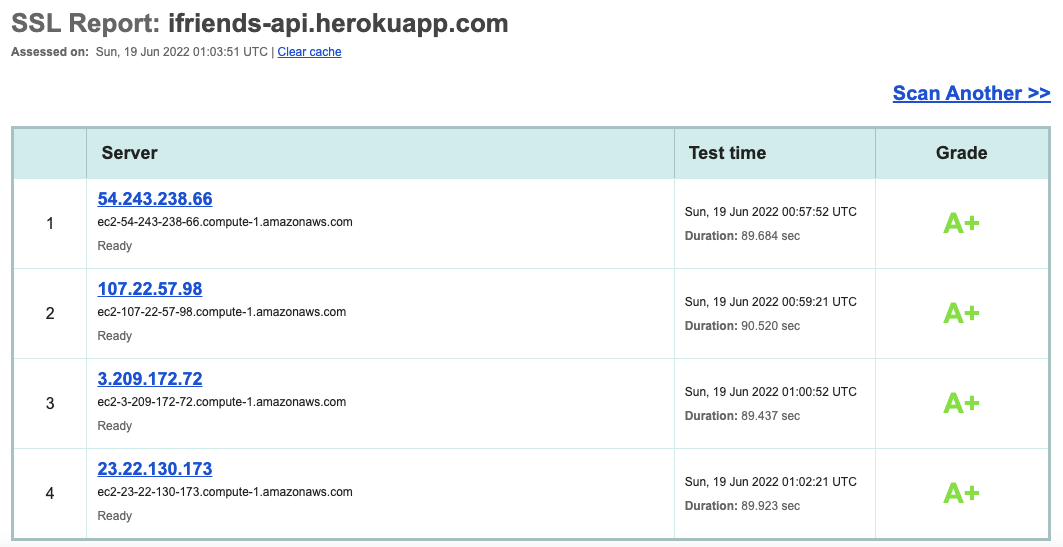
\includegraphics[width=1\textwidth]{anexos/Imagens_Seguranca/analise_ssllabs_api_heroku.png}
\fonte{os autores}
\end{figure}
\FloatBarrier

A análise completa do que está descrito na \autoref{analise_ssllabs_api_heroku} também se encontra disponível para visualização \href{https://www.ssllabs.com/ssltest/analyze.html?d=app-ifriends.herokuapp.com}{aqui}.

\begin{figure}[htb]
\centering
\caption{\label{analise_ssllabs_frontend_heroku} Análise de segurança no Front-end}
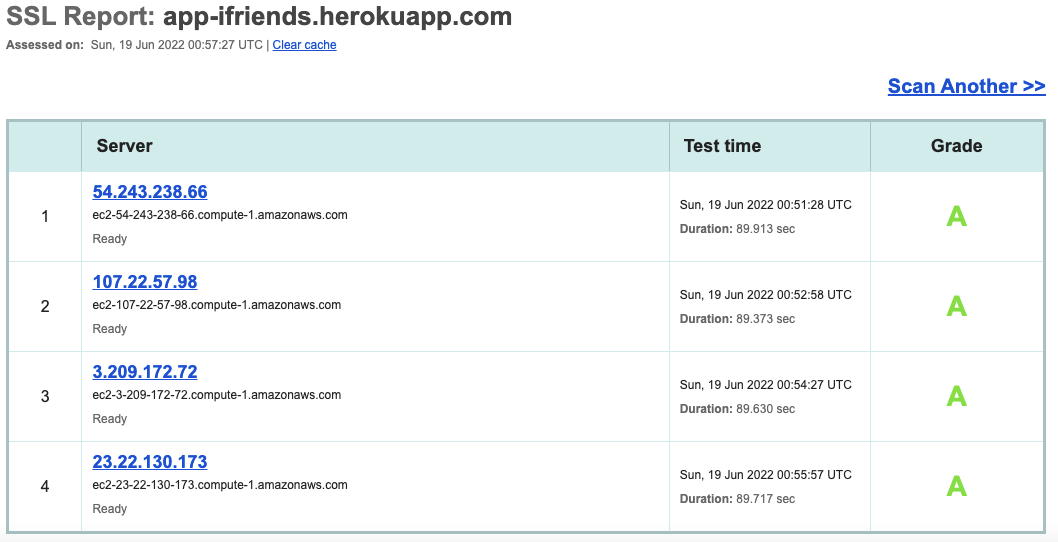
\includegraphics[width=1\textwidth]{anexos/Imagens_Seguranca/analise_ssllabs_frontend_heroku.png}
\fonte{os autores}
\end{figure}
\FloatBarrier

A análise completa do que está descrito na  \autoref{analise_ssllabs_frontend_heroku} também se encontra disponível para visualização \href{https://www.ssllabs.com/ssltest/analyze.html?d=ifriends-api.herokuapp.com}{aqui}.

Além disso, conforme os requisitos da disciplina, a \acs{api} teve suas respostas \acs{http} analisadas pelo \href{https://securityheaders.io}{\textit{Security Headers}}, e conforme observado na \autoref{analise_http_response_api}, a aplicação conseguiu configurar todos os cabeçalhos básicos de segurança requeridos na análise.

\begin{figure}[htb]
\centering
\caption{\label{analise_http_response_api} Análise de respostas HTTP na API}
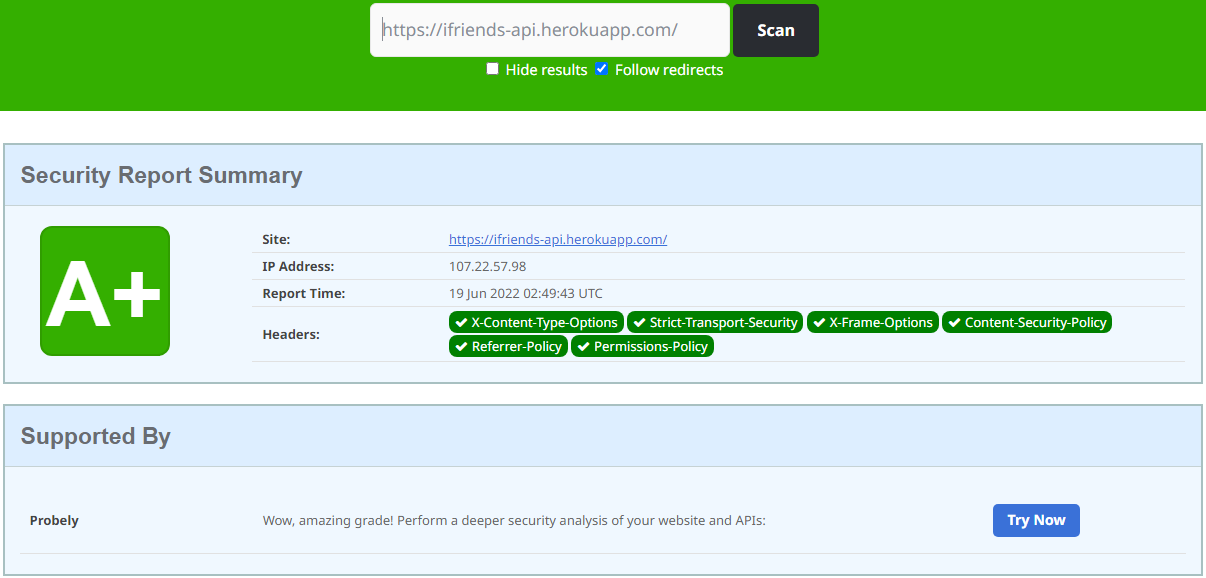
\includegraphics[width=1\textwidth]{anexos/Imagens_Seguranca/analise_http_response_api.png}
\fonte{os autores}
\end{figure}
\FloatBarrier

Ainda assim, na procura por alternativas ao Heroku, a equipe pôde verificar que alguns servidores oferecem suporte completo ao \acs{tls} de forma gratuita, como o caso do \href{https://vercel.com/blog/automatic-ssl-with-vercel-lets-encrypt}{Vercel} para o lado do cliente. Já para o servidor, a única alternativa encontrada é criar os certificados manualmente e renová-los a cada três meses (para o cliente, esta também é uma possibilidade), porém a praticidade de hospedagem disponibilizada pelo \gls{heroku} nesse caso, com \acs{sgbd} já nativo no servidor, é um dos desafios que dificultariam a migração para um novo serviço de hospedagem. De todo modo, cabe uma nova investigação dos meios para atender aos requisitos da disciplina.
